% !TeX spellcheck = en_US
\documentclass[french]{yLectureNote}

\title{Mecanique Analytique}
\subtitle{Physique}
\author{Paulhenry Saux}
\date{\today}
\yLanguage{Français}
%lionels.calmels@cemes.fr
\professor{M.Brut}
\usepackage{graphicx}%----pour mettre des images
\usepackage[utf8]{inputenc}%---encodage
\usepackage{geometry}%---pour modifier les tailles et mettre a4paper
%\usepackage{awesomebox}%---pour les boites d'exercices, de pbq et de croquis ---d\'esactiv\'e pour les TP de PC
\usepackage{tikz}%---pour deiffner + d\'ependance de chemfig
% \usepackage{tabularx}%---pour dimensionner automatiquement les tableaux avec variable X
\usepackage{awesomebox}%---Pour les boites info, danger et autres
\usepackage{menukeys}%---Pour deiffner les touches de Calculatrice
\usepackage{fancyhdr}%---pour les en-t\^ete personnalis\'ees
\usepackage{blindtext}%---pour les liens
\usepackage{hyperref}%---pour les liens (\`a mettre en dernier)
\usepackage{caption}%---pour la francisation de la l\'egende table vers Tableau
\usepackage{pifont}
\usepackage{array}%---pour les tableaux
\usepackage{lipsum}
\usepackage{yFlatTable}
\usepackage{multicol}
\usepackage{tabularx}
\usepackage{booktabs}
\newcommand{\Lim}[1]{\lim\limits_{\substack{#1}}\:}
\renewcommand{\vec}{\overrightarrow}
\newcommand{\N}[0]{\mathbb{N}}
\newcommand{\dd}{\mathrm{d}}
\newcommand{\norm}[1]{||\vec{#1}||}
\newcommand{\fo}{\psi(\vec{r},t)}
\newcommand{\foe}{\psi(\vec{r},t)\*}
\newcommand{\HH}{\hat{H}}
\newcommand{\hb}{\hbar}
\newcommand{\lap}{\nabla^2}
\newcommand{\lapcc}{\frac{\partial^2 }{\partial x^2}+\frac{\partial^2 }{\partial y^2}+\frac{\partial^2 }{\partial z^2}}
\newcommand{\E}{\vec{E}(M)}
\newcommand{\B}{\vec{B}(M)}
\newcommand{\V}{V(M)}
\newcommand{\er}{\vec{e_{\rho}}}
\newcommand{\ep}{\vec{e_{\varphi}}}
\newcommand{\pip}{\pi^+}
\newcommand{\pim}{\pi^-}
\newcommand{\mv}{\mathcal{V}}
\DeclareMathOperator{\Div}{Div}
\newcommand{\rot}{\vec{\mathrm{rot}}}
\newcommand{\grad}{\vec{\mathrm{grad}}}
\newcommand{\qa}{q_{\alpha}}
\newcommand{\qdb}{\dot{q_{\beta}}}
\newcommand{\qb}{q_{\beta}}
%\setcounter{chapter}{3}
\begin{document}
\chapter{Mécanique lagrangienne}
\section{Introduction}
\subsection{Pourquoi la mécanique Lagrangienne ?}
\subsubsection{Travailler avec des scalaires}
On prend l'exemple de l'oscillateur harmonique. On utilise une approche énergétique :
\begin{flalign*}
    E_m &= \frac12 \dot{x}^2+\frac12 kx^2\\
    \frac{\dd}{\dd t}E_m &=0\\
    &\iff (m\ddot{x}+kx)\dot{x} =0
\end{flalign*}
On obtient l'équation du mouvement, qui est scalaire.
\subsubsection{Travailler avec des systèmes contraints}
On prend l'exemple du pendule de masse m accrochée à un fil de longueur l.

Il faudrait 2 coordonnées indépendant mais une seule car le système est contraint par $ x^+y^⁼l^2$. On prend alors l'angle $\varphi$ comme unique coordonnée.

Cela s'applique aussi en dimension supérieure, comme dans le cas d'une particule dans une sphère. On peut alors écrire la contrainte :
$$x^2+y^2+z^2 = R^2$$
On n'utilise que 2 variables, avec le système de coordonnées sphériques


\includegraphics[scale=0.5]{s1}

\subsection{Contraintes}
\subsubsection{Définitions}
On se place dans un système dans un espace en D dimensions de coordonéees $x_1,\dots, x_n$\marginCritical{Cela ne correspond pas nécéssairement aux coordonnées de l'espace. Si on étudie 2 particules, cela correspond à la somme des degrés de libertés des 2 particules.}
\begin{definition}[Contrainte holonome]
     On étudie une contrainte qui s'écrit de la forme $$f(x_1,\dots,x_n,t) = 0$$
    \begin{itemize}
        \item Si $f$ ne dépend pas du temps, c'est une contrainte holon\^ome scléron\^ome
        \item Si il y a une dépendance selon $t$, elle est dite rhéon\^ome
    \end{itemize}
\end{definition}
\begin{proposition}[Degrés de libertés]
    Un système déterminé par $D$ coordonnées indépendantes mais soumis à $k$ contraintes holonômes indépendantes
a $N = D - k$ degrés de liberté.
\end{proposition}
Il faut donc N coordonnées généralisées indépendante
pour décrire entièrement le système. 
\warningInfo{Contraintes indépendantes}{
    On construit la matrice des dérivées partielles $$(\frac{\partial f_1}{\partial x_1}\dots \frac{\partial f_1}{\partial x_D}// \frac{\partial f_k}{\partial x_1} \dots \frac{\partial f_k}{\partial x_D})$$
}
\subsubsection{Exemple}
\begin{multicols}{2}


\includegraphics[scale=0.4]{s2}
\columnbreak

Si on prend un exemple 3D avec une contrainte, je peux imaginer un sous-espace dans lequel le système peut évoluer. On pourra alors prendre des coordonnées adpatées à ce sous-espace, u et v.
\end{multicols}

On peut écrire $\frac{\partial X}{\partial u}$ et $\frac{\partial X}{\partial v}$ sont tangents à la surface.

On peut aussi trouver un vecteur orthogonal\marginInfo{On peut aussi faire avec le produit vectoriel de u et v} à la surface en sachant que 
$$\frac{\dd }{\dd t}f(\vec{X}(t)) = 0\Rightarrow \dot{\vec{X}}\cdot \vec{\nabla}f =0$$

\section{Lois de Newton et d'Euler-Lagrange}
Soit un système de D dimensions et soumis à k contraintes indépendantes. Le système est soumis aux forces conservatrices $\vec{F_1},\dots, \vec{F_n}$, dont la somme vaut $\vec{F_{ext}}$. On suppose que le mouvement se fait sans frottements

On peut écrire $\vec{F_{ext}} = -\vec{\nabla}V$ avec $V$ l'énergie potentielle associée.

De plus, les forces $\vec{F_{x_k}}$ sont les forces qui maintiennent les contraintes\marginTips{Par exemple, la force de tension du fil qui maintient la masse à une distance l de l'origine, ou encore la réaction du support.}.

\begin{theorem}[Principe d'Almebert]
    Il y a k forces $\vec{F_{C_i}}$ pour satisfaire les contraintes $f_i(\vec{x})=0$ pour un mouvement sans frottement. Alors 
    $$\vec{F_{C_i}}\propto \vec{\nabla}f_i$$
\end{theorem}
On peut donc écrire $$\sum_i^k \vec{F_{x_i}} = \sum_i^k \lambda_i \vec{\nabla}f_i$$
\subsection{Conséquences}
\subsubsection{f schléronôme}
Si  $f_i$ est schléronôme ; $\vec{\nabla}f_i$ est un vecteur orthogonal au sous espace donnée par $f_i = 0$.

On a donc 
$$\frac{\dd }{\dd t}f_i(\vec{x},t)=0 \iff \vec{\nabla}f\cdot \dot{\vec{x}} = 0$$

On en déduit que la forces de contraintes ne travaille pas\marginTips{En effet, $\vec{F_c}$ est orthogonal au sous-espace, et par définition, le travail est nul ($\vec{F_C}\cdot \vec{v} = 0)$}.

\subsubsection{f rhéon\^ome}
On étudie la trajectoire d'une fourmi sur un ballon. On gonfle le balon pendant que la fourmi en fait le tour.

$\dd \vec{x}$ est le déplacement réel du ballon et $\delta \vec{x}$ le déplacement virtuel de la particule. 
La particule a donc un déplacement $\Delta \vec{x} = \dd \vec{x}+\delta \vec{x}$.

\begin{proposition}[Condition de non frottement]
    $$\vec{F_c}\perp \delta \vec{x}$$ $\vec{F_c}$ est orthogonal à la surface, donc $\vec{F_C}\propto \vec{\nabla}f$.
\end{proposition}
\criticalInfo{Forces de contriantes}{Dans les deux cas, elles sont orthognales à la surface de déplacement.}
\subsection{lois fondamentales}
On reprend l'exemple avec une particule évoluant dans le sous espace de la nappe. Le SE a N vecteurs tangents $\tau_{\alpha} = \frac{\partial \vec{x}}{\partial q_{\alpha}}$

On pose $\vec{F_C}$ la force de contrainte totale, qui est donc orthogonale.

On applique la LFD :
\begin{flalign*}
    m\ddot{\vec{x}} &= \vec{F_c}+\vec{F_{ext}}\\
    m\ddot{\vec{x}}\cdot \vec{\tau_\alpha} &= \vec{\tau_\alpha}\cdot \vec{F_{ext}} + \sum_{i^k } \lambda_i \vec{\nabla}f_i \cdot  \vec{\tau_\alpha}\\
    &= \vec{\tau_\alpha}\cdot \vec{F_{ext}}\\
\end{flalign*}
En se rapellant que $\tau_\alpha^i = \frac{\partial x_i}{q_\alpha}$, on écrit
\begin{flalign*}
    m\sum_i^D \ddot{x_i}\frac{\partial x_i}{_partial q_{\alpha}}-\sum_i^D F_{ext}\frac{\partial x_i}{\partial q_{\alpha}}\\
\end{flalign*}
Cependant, on peut réécrire :
\begin{flalign*}
    \vec{F_{ext}} = -\vec{\nabla} V\\
    \Rightarrow F_{ext}^i = -\frac{\partial V}{\partial x_i}\\
    \Rightarrow \sum_i^D F_{ext}^i \frac{\partial x_i}{\partial q_{\alpha}} = -\frac{\partial V}{\partial q_{\alpha}}
\end{flalign*}
On réécrit l'autre terme :
\begin{flalign*}
    \ddot{x_i}\frac{\partial x_i}{\partial q_{\alpha}}= \frac{\dd}{\dd t}(\dot{x_i}\frac{\partial x_i}{\partial qu_{\alpha}})-\dot{x_i}\frac{\dd}{\dd t}(\frac{\partial x_i}{\partial q_{\alpha}})\\
    \Rightarrow \frac{\partial \dot{x_i}}{\partial \dot{q_\alpha}} = \frac{\partial x_i}{\partial q_{\alpha}}
\end{flalign*}
On écrit maintenant 
\begin{flalign*}
    \frac{\dd }{\dd t}\sum m \dot{x_i}(\frac{\partial \dot{x_i}}{\partial \dot{q_{\alpha}}}) - \sum_i \dot{x_i}\frac{\partial \dot{x_i}}{\partial q_{\alpha}} + \frac{\partial V}{\partial q_{\alpha}} = 0
\end{flalign*}
\begin{definition}[Lagrangien]
    $$L(q_{\alpha}, \dot{q_{\alpha}}, t) = U-V = \frac12 m\ddot{x}^2-V$$
\end{definition}
\begin{theorem}[Équation d'Euler-Lagrange]
    $$\frac{\dd }{\dd t}(\frac{\partial L}{\partial \dot{q_{\alpha}}})-\frac{\partial L}{\partial q_{\alpha}} = 0$$
\end{theorem}
\section{Exemples}
\subsection{Pendule}
On reprend l'exemple de pendule. On a $f\vec{x} = x^2+y^2-l^2=0$

On peut écrire $x(\varphi) = l\cos(\varphi), y(\varphi)=l\sin(\varphi)$ En dérivant, on obtient $x(\varphi) = -l\sin(\varphi), y(\varphi)=l\cos(\varphi)$

Comme $\vec{v} = \dot{x}\vec{e_x}+\dot{y}\vec{e_y}$, on en déduit que $\vec{v}^2 = \dot{x}^2+\dot{y}^2 = l^2\dot{\varphi}^2$

De plus, dans la direction $\vec{P}$, on a $V_{P} = -mgl\cos(\varphi)$ en appliquant le PFD.

On peut maintenant écrire le Lagrangien : $$\frac12 ml^2\dot{\varphi}^2+mgl\cos(\varphi)$$


\warningInfo{Résumé}{On a un système de coordonnées $\chi_i$ et k contraintes indépendantes. On a fonc $N=D-k$ coordonnées généralisées $q_{_alpha}$.

On a $$U = E_c = \frac12 m \sum_i (\dot{x_i}^2) = U(q_{\alpha}; \dot{q_{\beta}}^2,t)$$
et
$$V = E_p = V(q_{\alpha},t)$$
puis 
$$L = E_c-E_p = U-V$$
On obtient l'équation d'Euler-Lagrange :
 $$\frac{\dd }{\dd t}(\frac{\partial L}{\partial \dot{q_{\alpha}}})-\frac{\partial L}{\partial q_{\alpha}} = 0$$
 On a pour chaque $\alpha$ l'EQD ci-dessus.
}
\subsection{oscillateur harmonique}
\begin{multicols}{2}

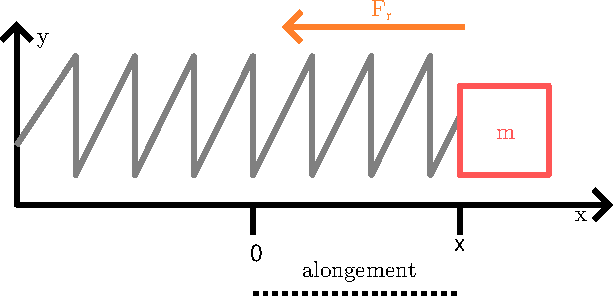
\includegraphics[scale=0.5]{oss.pdf}
\columnbreak
Dans cette situation, on obtient 
\end{multicols}
$$L(x\dot{x}) = \frac12 m\dot{x}^2-\frac12 Kx^2$$
En appliquant Euler-lagrange, on a 
$$m\ddot{x}+Kx =0$$ qui est un oscillateur harmonique
\subsection{Pendule 3-D}
\begin{multicols}{2}


\includegraphics[scale=0.5]{pendule.pdf}
\columnbreak

On a la contrainte $x_1^2+x_2^2+x_3^3-R^2=0$.

On peut écrire :
\begin{flalign*}
x_1 &= R\sin\theta \cos\varphi\\
x_2 &= R\sin \theta \sin \varphi\\
x_3 &= R\cos\theta\\
\end{flalign*}

\end{multicols}


On dérive :
\begin{flalign*}
\dot{x_1} &= R\dot{\theta}\cos\theta\cos\varphi - R\dot{\varphi}\sin\theta\sin\varphi\
\dot{x_2} &= R\dot{\theta}\cos\theta\sin\varphi + R\dot{\varphi}\sin\theta\cos\varphi\
\dot{x_3} &= -R\dot{\theta}\sin\theta\
\end{flalign*}
On en déduit :
$$\dot{x_1}^2+\dot{x_2}^2+\dot{x_3}^2 = R\dot{\theta}^2+R\dot{\varphi}^2\sin^2(\theta)$$
On peut maintenant calculer le lagrangien :
$$L(\theta,\varphi, \dot{\theta}, \dot{\varphi}) = \frac12 mR^2\dot{\theta}^2+\frac12 m R^2 \sin^2(\theta)\dot{\varphi}^2 - mgR\cos(\theta)$$

En appliquant Euler-lagranges, on obtient 2 équations :
\begin{flalign*}
    mR^2 \ddot{\theta}-mgR\sin\theta-mR^2\sin\theta \cos\theta \dot{\varphi}^2&=0\\
    2mR^2\cos\theta\sin\theta \dot{\theta}\dot{\varphi}+mR^2\sin^2\theta\ddot{\varphi}&=0
\end{flalign*}
On en déduit que $mR^2\sin^2\theta\dot{\varphi} = Cst = L_z$.
\subsection{Bille}
\begin{multicols}{2}
\centering
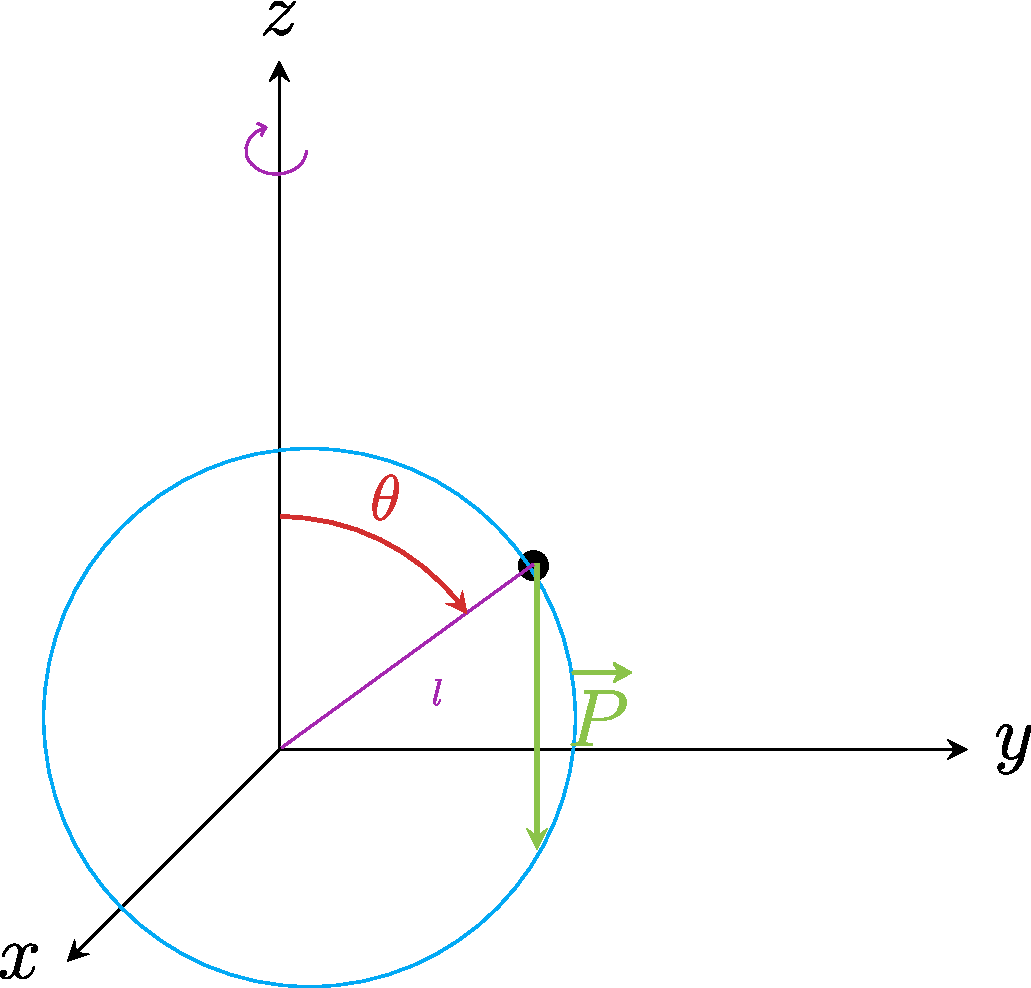
\includegraphics[scale=0.3]{bille}
\columnbreak

On a ici 2 contraintes scléronomes :

\begin{itemize}
    \item $x_1^2+x_2^2+x_3^3-R^2=0$
    \item $x_2-x_1tg(\omega t) = 0$
\end{itemize}
\end{multicols}

On a $\vec{P} = -mg\vec{e_z}\Rightarrow V = mgR\cos(\theta)$

De plus, $U = \frac12 mv^2 = \frac12m(R^2\dot{\theta}^2+R^2\omega^2\sin^2\theta)$

On peut écrire le lagrangien puis avec Euler-Lagrange :
$$mR^2\ddot{\theta}-mR^2\omega^2\sin(\varphi)\cos(\varphi)-mgR\sin(\theta) = 0$$
\subsection{Machine d'Atwood}
\begin{multicols}{2}
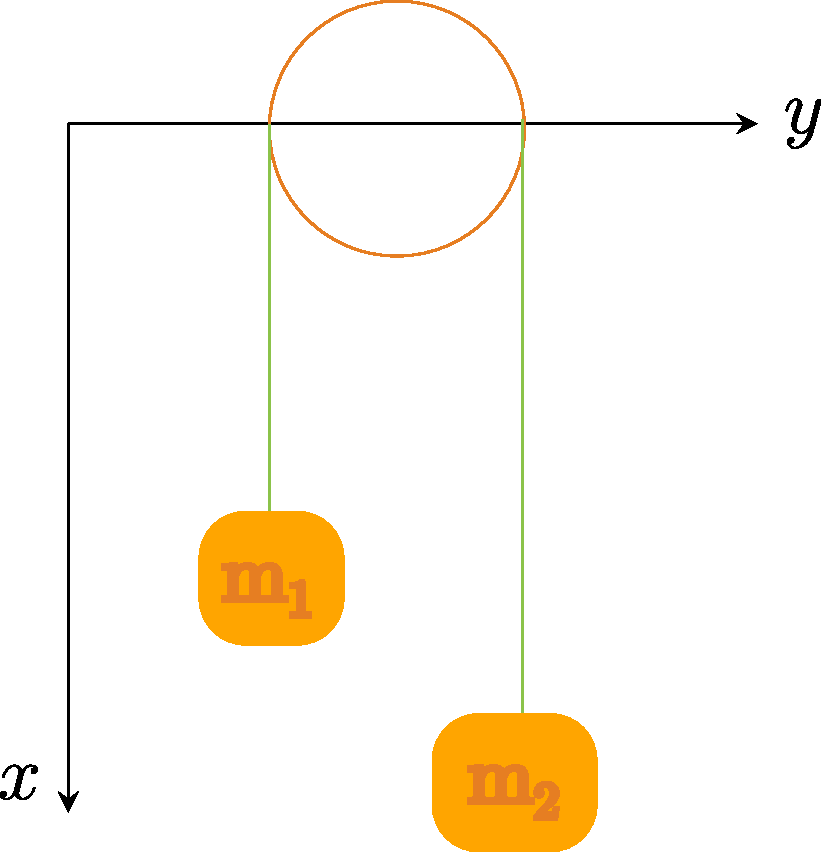
\includegraphics[scale=0.25]{masses.pdf}
\columnbreak

On a une corde statique de longueur $l+\pi D$

On a $x_1+x_2-l=0$, $z_1=z_2 = 0$ et $y_1, y_2= Cst$.

\end{multicols}

On écrit 
$$V = E_p = -mgx_1-m_2gx_2 = -(m_1-m_2)g_x1-m_2gl$$
et 
$$ U=E_c = \frac{1}{2} m_1\dot{x_1^2}+\frac12 m_2\dot{x_2}^2 = \frac12(m_1+m_2)$$
Euler-Lagrange donne 
$$(m_1+m_2)\ddot{x_1}=(m_1-m_2)g$$
\criticalInfo{Observations importantes}{
    Soit L un  lagrangien $$L_1(q_{\alpha},\dot{q_{beta}},t)$$ et $$L_2(q_{\alpha},\dot{q_{beta}},t) = L_1(q_{\alpha},\dot{q_{beta}},t) + \frac{\dd}{\dd t}F(_{\alpha},t)$$

    Avec $$\frac{\dd}{\dd }F = \frac{\partial F}{\partial t} F \sum_{\alpha}\frac{\partial F}{\partial q_{\alpha}}\dot{q_{\alpha}}$$

    Alors $L_1$ et $L_2$ donnent les m\^emes équations du mouvement.
}
% \begin{myproof}
%     Il suffit de montrer que $\frac{\dd}{\dd t}(\frac{\partial}{\partial \dot{q_{\alpha}}}(\frac{\dd}{\dd t}F))-\frac{\partial }{\partial q_{\alpha}}(\frac{\dd F}{\dd t})=0\forall \beta$

%     On a $\frac{\partial}{\partial \dot{q_{\beta}}} = \frac{\partial F}{\partial q_{\beta}}$

%     %OK Finir demo

% \end{myproof}

\begin{myproof}
    Il suffit de montrer que $\frac{\dd}{\dd t}\left(\frac{\partial}{\partial \dot{q}_{\beta}}\left(\frac{\dd F}{\dd t}\right)\right)-\frac{\partial }{\partial q_{\beta}}\left(\frac{\dd F}{\dd t}\right)=0 \quad \forall \beta$.

    Calculons séparément chaque terme en utilisant l'expression de la dérivée totale de $F$ :
    $$\frac{\dd F}{\dd t} = \frac{\partial F}{\partial t} + \sum_{\alpha} \frac{\partial F}{\partial q_{\alpha}}\dot{q}_{\alpha}$$

    1) Pour le premier terme, on dérive par rapport à $\dot{q}_{\beta}$. Comme $F$ ne dépend que de $q_{\alpha}$ et $t$, les dérivées partielles $\frac{\partial F}{\partial t}$ et $\frac{\partial F}{\partial q_{\alpha}}$ sont indépendantes des vitesses. Seul le terme de la somme où $\alpha = \beta$ subsiste :
    $$\frac{\partial}{\partial \dot{q}_{\beta}} \left( \frac{\dd F}{\dd t} \right) = \frac{\partial F}{\partial q_{\beta}}$$
    En prenant la dérivée temporelle totale de ce résultat, on obtient :
    $$\frac{\dd}{\dd t} \left( \frac{\partial F}{\partial q_{\beta}} \right) = \frac{\partial^2 F}{\partial t \partial q_{\beta}} + \sum_{\alpha} \frac{\partial^2 F}{\partial q_{\alpha} \partial q_{\beta}} \dot{q}_{\alpha}$$

    2) Pour le second terme, on dérive directement $\frac{\dd F}{\dd t}$ par rapport à $q_{\beta}$ :
    $$\frac{\partial}{\partial q_{\beta}} \left( \frac{\dd F}{\dd t} \right) = \frac{\partial^2 F}{\partial q_{\beta} \partial t} + \sum_{\alpha} \frac{\partial^2 F}{\partial q_{\beta} \partial q_{\alpha}} \dot{q}_{\alpha}$$

    D'après le théorème de Schwarz, les dérivées croisées sont égales ($\frac{\partial^2 F}{\partial t \partial q_{\beta}} = \frac{\partial^2 F}{\partial q_{\beta} \partial t}$ et $\frac{\partial^2 F}{\partial q_{\alpha} \partial q_{\beta}} = \frac{\partial^2 F}{\partial q_{\beta} \partial q_{\alpha}}$). Les deux termes sont donc identiques, ce qui implique :
    $$\frac{\dd}{\dd t}\left(\frac{\partial}{\partial \dot{q}_{\beta}}\left(\frac{\dd F}{\dd t}\right)\right) - \frac{\partial }{\partial q_{\beta}}\left(\frac{\dd F}{\dd t}\right) = 0$$
    La contribution de $\frac{\dd F}{\dd t}$ aux équations d'Euler-Lagrange est nulle.
\end{myproof}

De plus, Euler-Lagrange est équivalent pour n'importe quel système de coordonnée.
\subsection{Particule chargée en présence d'un champ EM}
On construit $\vec{E} = -\nabla(\varphi)-\frac{\partial \vec{A}}{\partial t}$ et $\vec{B} = \vec{\nabla}\wedge \vec{A}$

Comment on a une invariance de Jauge, différentes combinaisons de potentiels donnent les m\^eme champs.

L'équation du mouvement vaut alors $m\ddot{\vec{x}} = q\vec{E}+q\vec{V}\wedge \vec{B}$

Le lagrangien donne $L = \frac12 m \dot{\vec{r}}^2-q\varphi(\vec{r},t) + q\dot{\vec{e}}\cdot \vec{A}$

De cette façon, si $\varphi\o\varphi-\frac{\partial \Omega}{\partial t}, \vec{A}\to \vec{A}+\vec{\nabla}\Omega$, on a 
$L\to L + q\frac{\partial \Omega}{\partial t}+q\dot{\vec{r}}\cdot \vec{\nabla}\Omega = L+q\frac{\dd \Omega}{\dd t}$

% \checkInfo{Exercice Tenseur totalement antisymétrique de Levi Civita}{
% Exercice OK Montrer que : $(\vec{V}\wedge \vec{B})_i = \sum_{sp} \epsilon_{spi}V_sB_p$

% Exercice 2 OK  Montrer que : $\sum \epsilon_{lmp}\epsilon_{isp}=\delta_{li}\delta_{ms}-\delta_{ls}\delta_{mi}$
% }


\checkInfo{Exercice Tenseur totalement antisymétrique de Levi Civita}{
    \textbf{Exercice 1 :} Montrer que $(\vec{V}\wedge \vec{B})_i = \sum_{j,k} \epsilon_{ijk}V_jB_k$.

    \textbf{Exercice 2 :} Montrer que $\sum_{p} \epsilon_{ijp}\epsilon_{klp} = \delta_{ik}\delta_{jl} - \delta_{il}\delta_{jk}$ (Identité fondamentale).
}

\begin{myproof}[Démonstration Exercice 1]
    Par définition du produit vectoriel $\vec{W} = \vec{V} \wedge \vec{B}$ en coordonnées cartésiennes :
    \begin{itemize}
        \item $W_1 = V_2 B_3 - V_3 B_2$
        \item $W_2 = V_3 B_1 - V_1 B_3$
        \item $W_3 = V_1 B_2 - V_2 B_1$
    \end{itemize}
    En utilisant le symbole de Levi-Civita où $\epsilon_{123}=1$, $\epsilon_{132}=-1$ et $\epsilon_{ijk}=0$ si deux indices sont égaux, on peut condenser ces expressions :
    $$(\vec{V}\wedge \vec{B})_i = \sum_{j=1}^3 \sum_{k=1}^3 \epsilon_{ijk} V_j B_k$$
    Pour coller à la notation $\epsilon_{spi}V_sB_p$, on vérifie par permutation circulaire que $\epsilon_{ijk} = \epsilon_{jki} = \epsilon_{kij}$. Ainsi, $\epsilon_{ijk} = \epsilon_{jki}$, ce qui correspond bien à $\epsilon_{spi}$ avec $s=j$ et $p=k$.
\end{myproof}

\begin{myproof}[Démonstration Exercice 2]
    L'identité $\sum_{p} \epsilon_{ijp}\epsilon_{klp} = \delta_{ik}\delta_{jl} - \delta_{il}\delta_{jk}$ se démontre par l'analyse des cas :
    
    1. Si $i=j$ ou $k=l$, le membre de gauche est nul (propriété d'antisymétrie de $\epsilon$). Le membre de droite l'est aussi (ex: si $i=j$, $\delta_{ik}\delta_{il} - \delta_{il}\delta_{ik} = 0$).
    
    2. Si $\{i,j\} \neq \{k,l\}$, alors pour tout $p$, soit $\epsilon_{ijp}=0$ soit $\epsilon_{klp}=0$. Le produit est nul, et les deltas de Kronecker s'annulent également.
    
    3. Si $\{i,j\} = \{k,l\}$ avec $i \neq j$ :
    \begin{itemize}
        \item Cas $i=k$ et $j=l$ : Le membre de gauche devient $\sum_p (\epsilon_{ijp})^2$. Le seul terme non nul est celui où $p \neq i$ et $p \neq j$, donc $(\pm 1)^2 = 1$. Le membre de droite donne $\delta_{ii}\delta_{jj} - \delta_{ij}\delta_{ji} = 1\cdot 1 - 0 = 1$.
        \item Cas $i=l$ et $j=k$ : Le membre de gauche devient $\sum_p \epsilon_{ijp}\epsilon_{jip} = \sum_p \epsilon_{ijp}(-\epsilon_{ijp}) = -1$. Le membre de droite donne $\delta_{ij}\delta_{ji} - \delta_{ii}\delta_{jj} = 0 - 1 = -1$.
    \end{itemize}
    L'identité est donc vérifiée dans tous les cas.
\end{myproof}

On peut désormais écrire :
$$\frac{\partial L}{\partial \dot{r_i}} = m\vec{r_i}+qA_i$$ 

$$\frac{\partial L}{\partial {r_i}}= q\sum_j \dot{r_j} \frac{\partial A_j}{\partial r_i}-q\frac{\partial \varphi}{\partial r_i}$$

On en déduit que 

$$m\ddot{r_i} = -q(\frac{\partial A_i}{\dd t} + \frac{\partial \varphi}{\partial r_i})+ q(\sum_j \dot{r_j} \frac{\partial A_j}{\partial r_i} - \sum_j \frac{\partial A_i}{\partial r_j}\dot{r_j})$$

et 

$$B_K = \sum_{l,m}\epsilon_{lm}\frac{\partial A_m}{\partial r_l}$$

\end{document}

